\section{Metodologías de trabajo}

    Durante el trabajo de título, el alumno trabajo junto al equipo de \textit{TechOps}, el cual incluye a \textit{Hive} y al \textit{Customer Portal}, proyecto que pretende facilitar la visibilidad de los productos contratados y entregar información de manera transparente a los clientes de Beetrack. Este equipo, conformado por Tomás Burotto, Juan José Martinez y el alumno, utiliza herramientas y metodologías propias de desarrollos ágiles para sus proyectos, en específico, se utiliza \textit{Scrum} con \textit{Sprints} de dos semanas.
    
    \textit{Scrum} se define como ``...un proceso en que se llevan a cabo un conjunto de tareas de forma regular con el objetivo principal de trabajar de manera colaborativa, es decir, trabajo en equipo.'' \cite{scrum_definition}, siendo esta metodología la más utilizada hoy en día en el mundo de desarrollo. Un \textit{Sprint} se caracteriza por comenzar con un \textit{Sprint Planning}, en el cual se determinan las tareas que cada colaborador realizará en el período de tiempo establecido, asignándole a cada tarea lo que se denomina como puntos de esfuerzo. Estos últimos son una forma de medir cuánto tiempo o dificultad tiene cada tarea, de manera de poder mantener un nivel de tareas constante a lo largo de los diferentes ciclos e ir  afinando el nivel de carga que cada integrante del equipo puede abarcar.
    
    Tanto las tareas como los puntos de esfuerzos asignados a estas se encuentran ordenadas en un tablero \textit{Kanban}, el cual permite organizar las labores. En particular, en la empresa se utiliza Jira para llevar el seguimiento de las tareas, ciclos de desarrollo, documentación y especificación de las labores. Cada integrante del equipo junta los requerimientos que llegan a lo largo del ciclo y los escribe en el tablero para ser posteriormente asignados en el comienzo del próximo. En la figura \ref{fig:kanban} se puede ver un ejemplo de cómo se ve el tablero en Jira.
    
    \begin{figure}
        \centering
        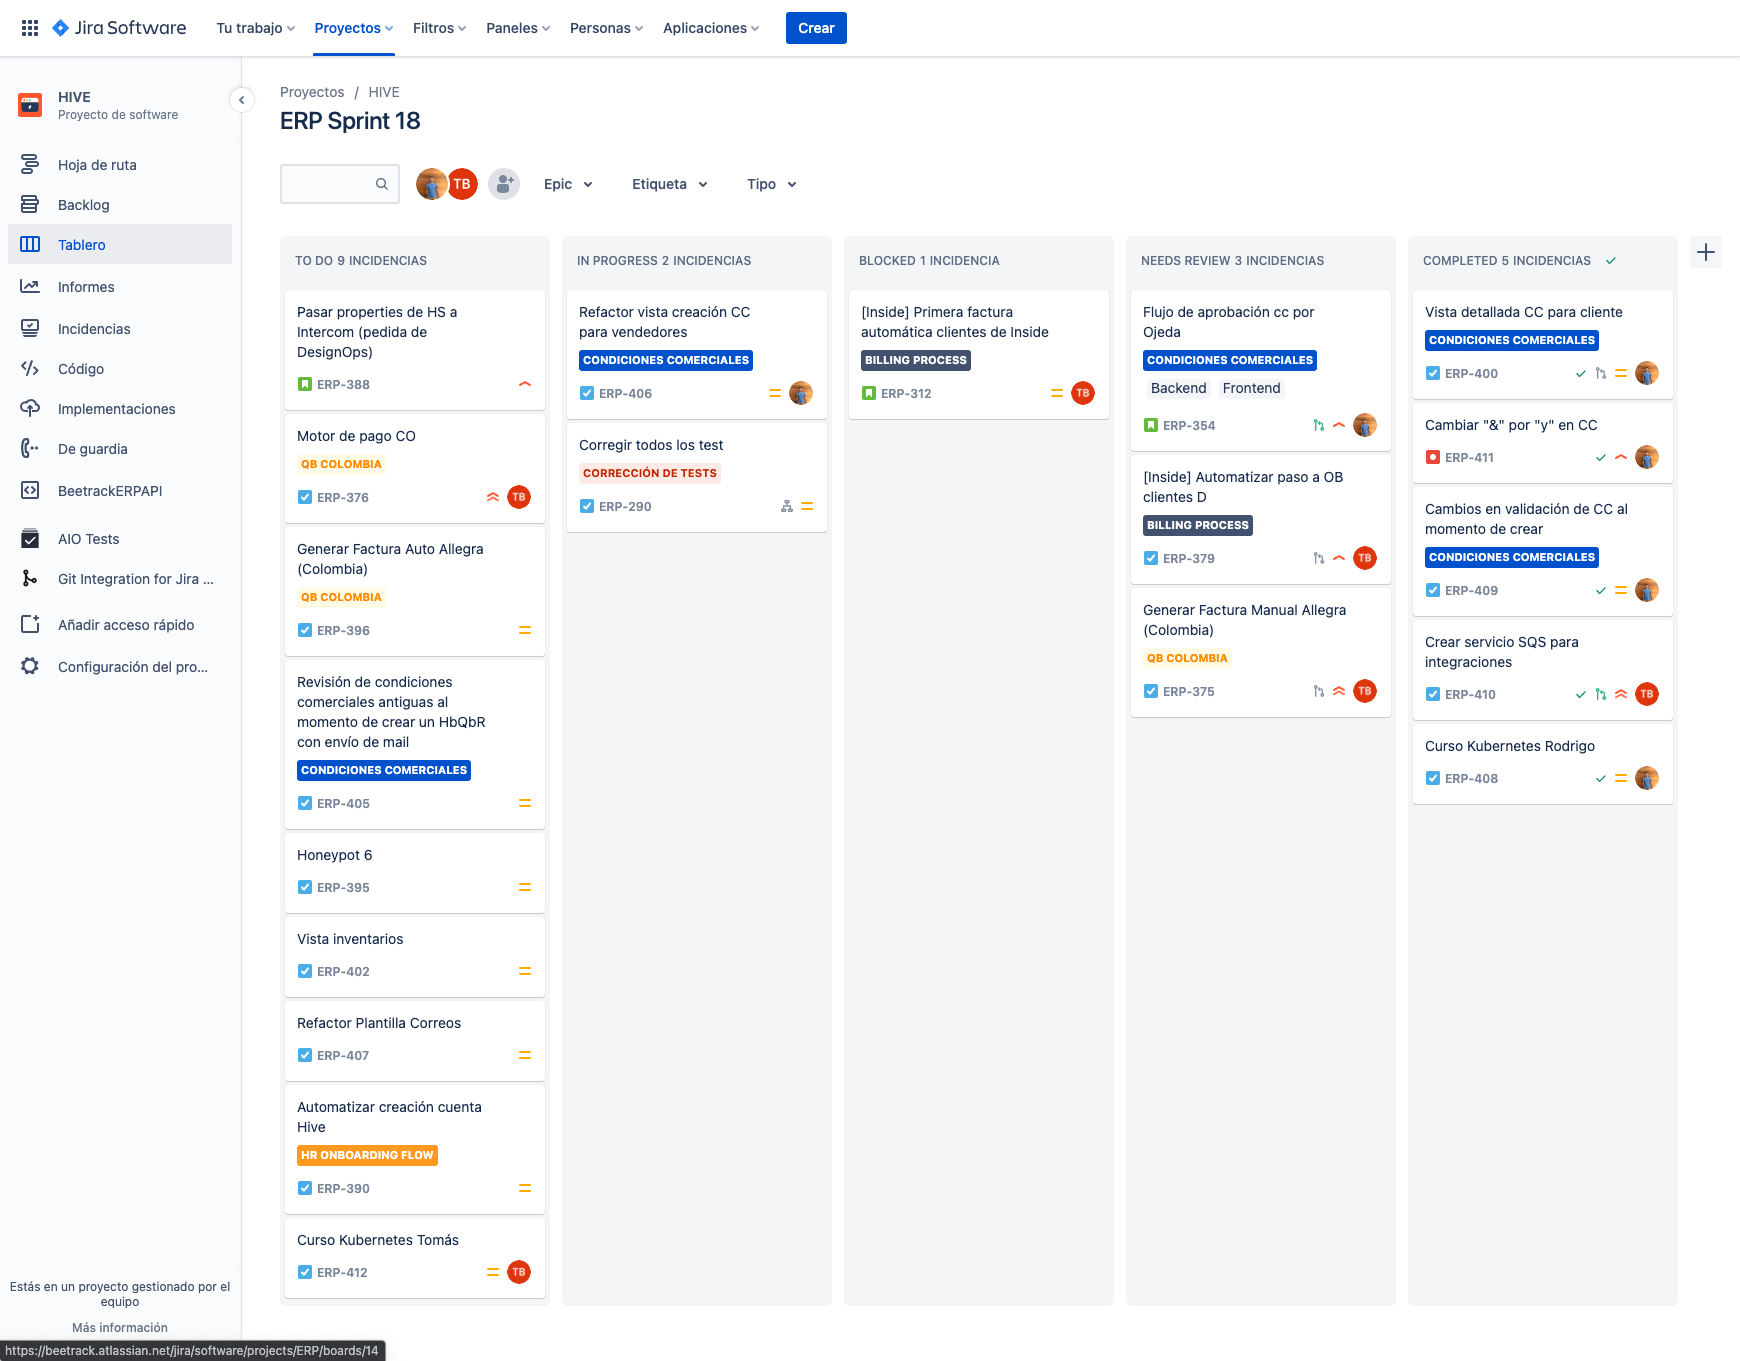
\includegraphics[width=0.75\linewidth]{figures/jira.png}
        \caption{Tablero \textit{Kanban} utilizado en el proyecto.}
        \label{fig:kanban}
    \end{figure}
    
    Debido a la cantidad de cambios que se deben realizar constantemente en el código, se requiere un versionamiento de este, por lo que se utiliza GitHub. Esta herramienta permite el uso de Git con \textit{Gitflow}. La principal ventaja de esta herramienta es que permite mantener diferentes versiones, como también utilizar un repositorio en donde se almacena el código en diferentes estados mediante \textit{branches}. Este uso de \textit{branches} o ``ramas'' permite mantener diferentes ambientes aislados uno del otro. El proyecto de \textit{Hive} cuenta con 3 ramas fijas, que nunca son eliminadas, \textit{master}, \textit{staging} y \textit{develop}. La primera rama es aquella que se encuentra en producción, es decir, es la que es visible para los usuarios finales, la segunda es un ambiente de pruebas (principalmente de estabilidad y de \textit{quality assurance}), y finalmente, la última es la rama de desarrollo, que es aquella en la cual se encuentra el código no probado por personas y que no se encuentra en ningún servidor de manera activa. 
    
    Cuando se quiere desarrollar una nueva funcionalidad, hacer correcciones o realizar cualquier tipo de cambio de código, la práctica es crear una nueva rama, hacer los cambios respectivos en el código, hacer una solicitud de cambio y revisión cruzada entre los miembros que tienen acceso al código, para finalmente integrar los cambios a la rama principal. En la figura \ref{fig:gitflow_diagram} se puede ver cómo se vería un diagrama de un flujo en Git.
    
    \begin{figure}
        \centering
        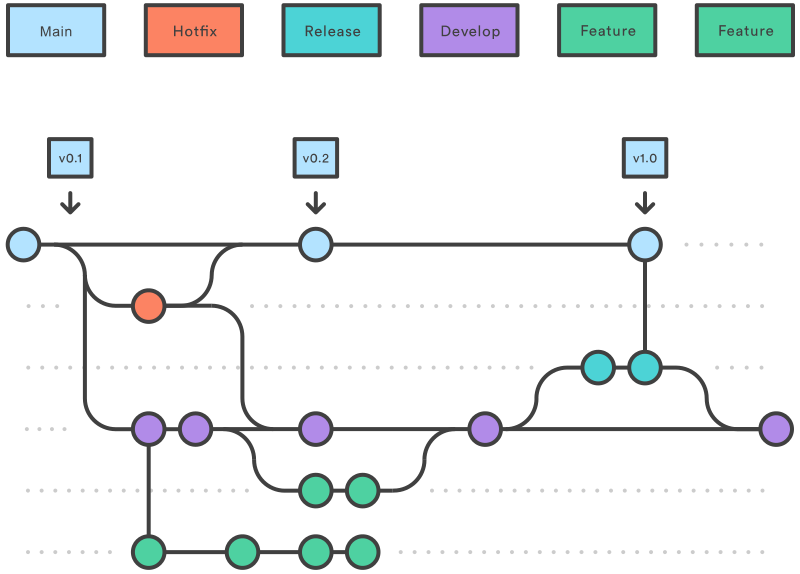
\includegraphics[width=0.65\linewidth]{figures/gitflow.png}
        \caption{\textit{Gitflow} \protect\cite{gitflow_diagram}.}
        \label{fig:gitflow_diagram}
    \end{figure}
    
    Finalmente, dentro de la empresa se utilizan procesos de integración continua, los cuales consisten en escritura de código que permite la puesta en producción del código que se subió a GitHub de manera automatizada en servidores remotos. En particular, se utiliza el SaaS Circle CI como intermediario. El flujo de integración continua, normalmente, comienza al subir el código a la rama \textit{master} o \textit{staging}, lo que gatilla una acción en los servidores de Circle CI, que descargan el código recién subido, corren pruebas sobre este, verifican su integridad, y finalmente compilan el código para subirlo a los servidores remotos especificados. La importancia de estas automatizaciones dentro de las metodologías de trabajo es que en el minuto en que estas automatizaciones fallan se despliegan alertas que permiten evitar que los servidores en producción se caigan por errores no previstos, sumado al hecho de que se permite ahorrar tiempo con tareas sistemáticas y bien establecidas. En la figura \ref{fig:continuous_integration} se puede ver el proceso descrito anteriormente.
    
    \begin{figure}
        \centering
        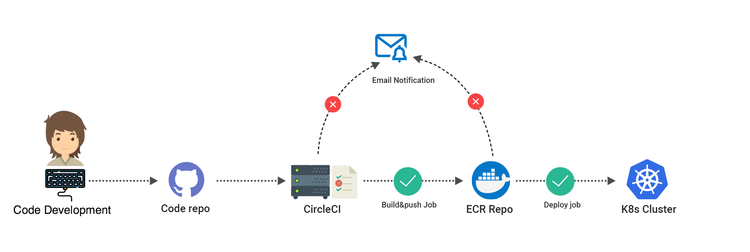
\includegraphics[width=0.9\linewidth]{figures/continuous_integration.png}
        \caption{Flujo de integración continua \protect\cite{continuous_integration}.}
        \label{fig:continuous_integration}
    \end{figure}

\section{Tecnologías utilizadas}

    El ERP de la empresa se basa en una arquitectura que separa de manera lógica los componentes. \textit{Hive} mismo tiene una separación entre \textit{frontend} y \textit{backend}, el primero corresponde a todo lo que concierne a la forma de visualizar e interactuar con la aplicación, mientras que el segundo se encarga de todas las operaciones y lógica de negocio de la aplicación, junto con sus interacciones. Estas dos partes se comunican mediante varios \textit{endpoints} a través de una API (\textit{Application Programming Interface}) que el \textit{backend} expone. 
    
    Por un lado, una API es un conjunto de definiciones y protocolos que se utiliza para desarrollar e integrar el software de las aplicaciones \cite{redhat_api}. Por otro lado, un \textit{endpoint} es una URL (\textit{Uniform Resource Locator}), o punto de acceso, mediante el cual una aplicación, o API, puede utilizar para obtener recursos y comunicarse con otra aplicación. En el caso del ERP, los \textit{endpoints} cuentan con una capa de seguridad para evitar accesos indeseados de aplicaciones no verificadas, teniendo que identificarse con un JWT (\textit{JSON Web Token}), el cual funciona como llave de acceso para la API y el \textit{backend}. En particular, se utiliza la librería Devise para generar los JWT que son utilizados por la aplicación \textit{frontend} y son únicos por sesión de usuario.
    
    El \textit{backend} de la aplicación está desarrollado en el lenguaje Ruby con el \textit{framework} Rails, por lo que se denomina \textit{Ruby on Rails} (o RoR). Este \textit{framework} permite construir aplicaciones rápidamente que sigan los patrones de diseño de ingeniería de \textit{software} de manera muy simple y que puedan escalar rápidamente. El patrón más utilizado por este \textit{framework} es el MVC (Modelo Vista Controlador), el cual divide a la aplicación en las tres partes mencionadas. En primer lugar, el modelo es un conjunto de clases que representan la información del mundo real que el sistema debe procesar. En segundo lugar, las vistas son el conjunto de clases que se encargan de mostrar al usuario la información contenida en el modelo. Finalmente, el controlador es un objeto que se encarga de dirigir el flujo del control de la aplicación debido a mensajes externos, como datos introducidos por el usuario u opciones del menú seleccionadas por él \cite{mvc_architecture}.
   
   En particular, para almacenar los datos de largo plazo de los modelos se utiliza una base de datos con un motor PostgreSQL (o PSQL). Cabe mencionar que no todos los datos se almacenan en este tipo de memoria y que no todas las operaciones se pueden realizar con esta. Es por lo anterior que también se hace uso de Sidekiq, una librería que permite la ejecución de tareas de manera asíncrona y/o en una fecha determinada mediante el almacenamiento de los datos necesarios en memoria \textit{caché}, para lo que se utiliza el motor Redis.
   
   Dada la naturaleza del ERP, como se mencionó anteriormente, este interactúa con otros servicios de dos maneras. Por un lado, para el servicio de condiciones comerciales, proyecto que el alumno realizó, se utiliza GraphQL, mientras que para el resto de los servicios, tales como Hubspot y Quickbooks, entre otros, se utilizan APIs REST. Una API REST es una API que se ajusta a los principios de diseño de REST, un estilo de arquitectura también denominado transferencia de estado representacional \cite{ibm_api_rest}. Este estilo es uno de los más populares para hacer APIs, pero es menos flexible al compararlo con GraphQL. Este último, es un lenguaje de consultas y servicio para APIs que prioriza el entregar a los consumidores exactamente la información solicitada y no más que eso. El principio de este lenguaje es hacer las APIs más flexibles, rápidas y posicionarse como alternativa a REST \cite{def_graphql}.
   
   El \textit{frontend} de \textit{Hive} está desarrollado en JavaScript con el \textit{framework} React. El código está construido sobre el principio de componentes reusables en las diferentes partes de la aplicación de manera de seguir el principio DRY (\textit{Don't Repeat Yourself}). Dado que el \textit{frontend} es aquel con el cual los usuarios interactúan, este requiere estilo, el cual está dado por el \textit{desing system, Honeypot}, de Beetrack. Este sistema de diseño es utilizado en todas las aplicaciones de la empresa de manera de que se pueda mantener una consistencia visual y de usabilidad entre las diferentes partes que componen los \textit{softwares} que se producen dentro de la empresa. En particular, este \textit{design system} abarca elementos como paleta de colores, diseños visuales de botones, formularios y componentes, entre otros, mientras que al mismo tiempo se tratan como paquetes prehechos, lo que permite reutilizarlos.
   
   En último lugar, tanto la aplicación de \textit{Hive} como el servicio de condiciones comerciales están alojadas en GKE (Google Kubernetes Engine). Este servicio permite mantener las aplicaciones mediante imágenes compiladas de Docker en servidores que son fácilmente escalables tanto vertical como horizontalmente mediante \textit{pods}, mientras que al mimso tiempo se encarga de los procedimientos para generar estos servidores y que se coordinen entre ellos. Los \textit{pods} son los objetos más pequeños y básicos que se pueden implementar en Kubernetes y representan una instancia única de un proceso en ejecución \cite{gke_pods}. Otra ventaja que provee GKE es la facilidad para poder volver imágenes que ya no se encuentran en uso en el caso de que ocurra algún error, lo que permite aumentar la disponibilidad del servicio entregado. En la figura \ref{fig:arquitectura} se puede ver la arquitectura con la cual el alumno trabajó.

  \begin{figure}
    \centering
    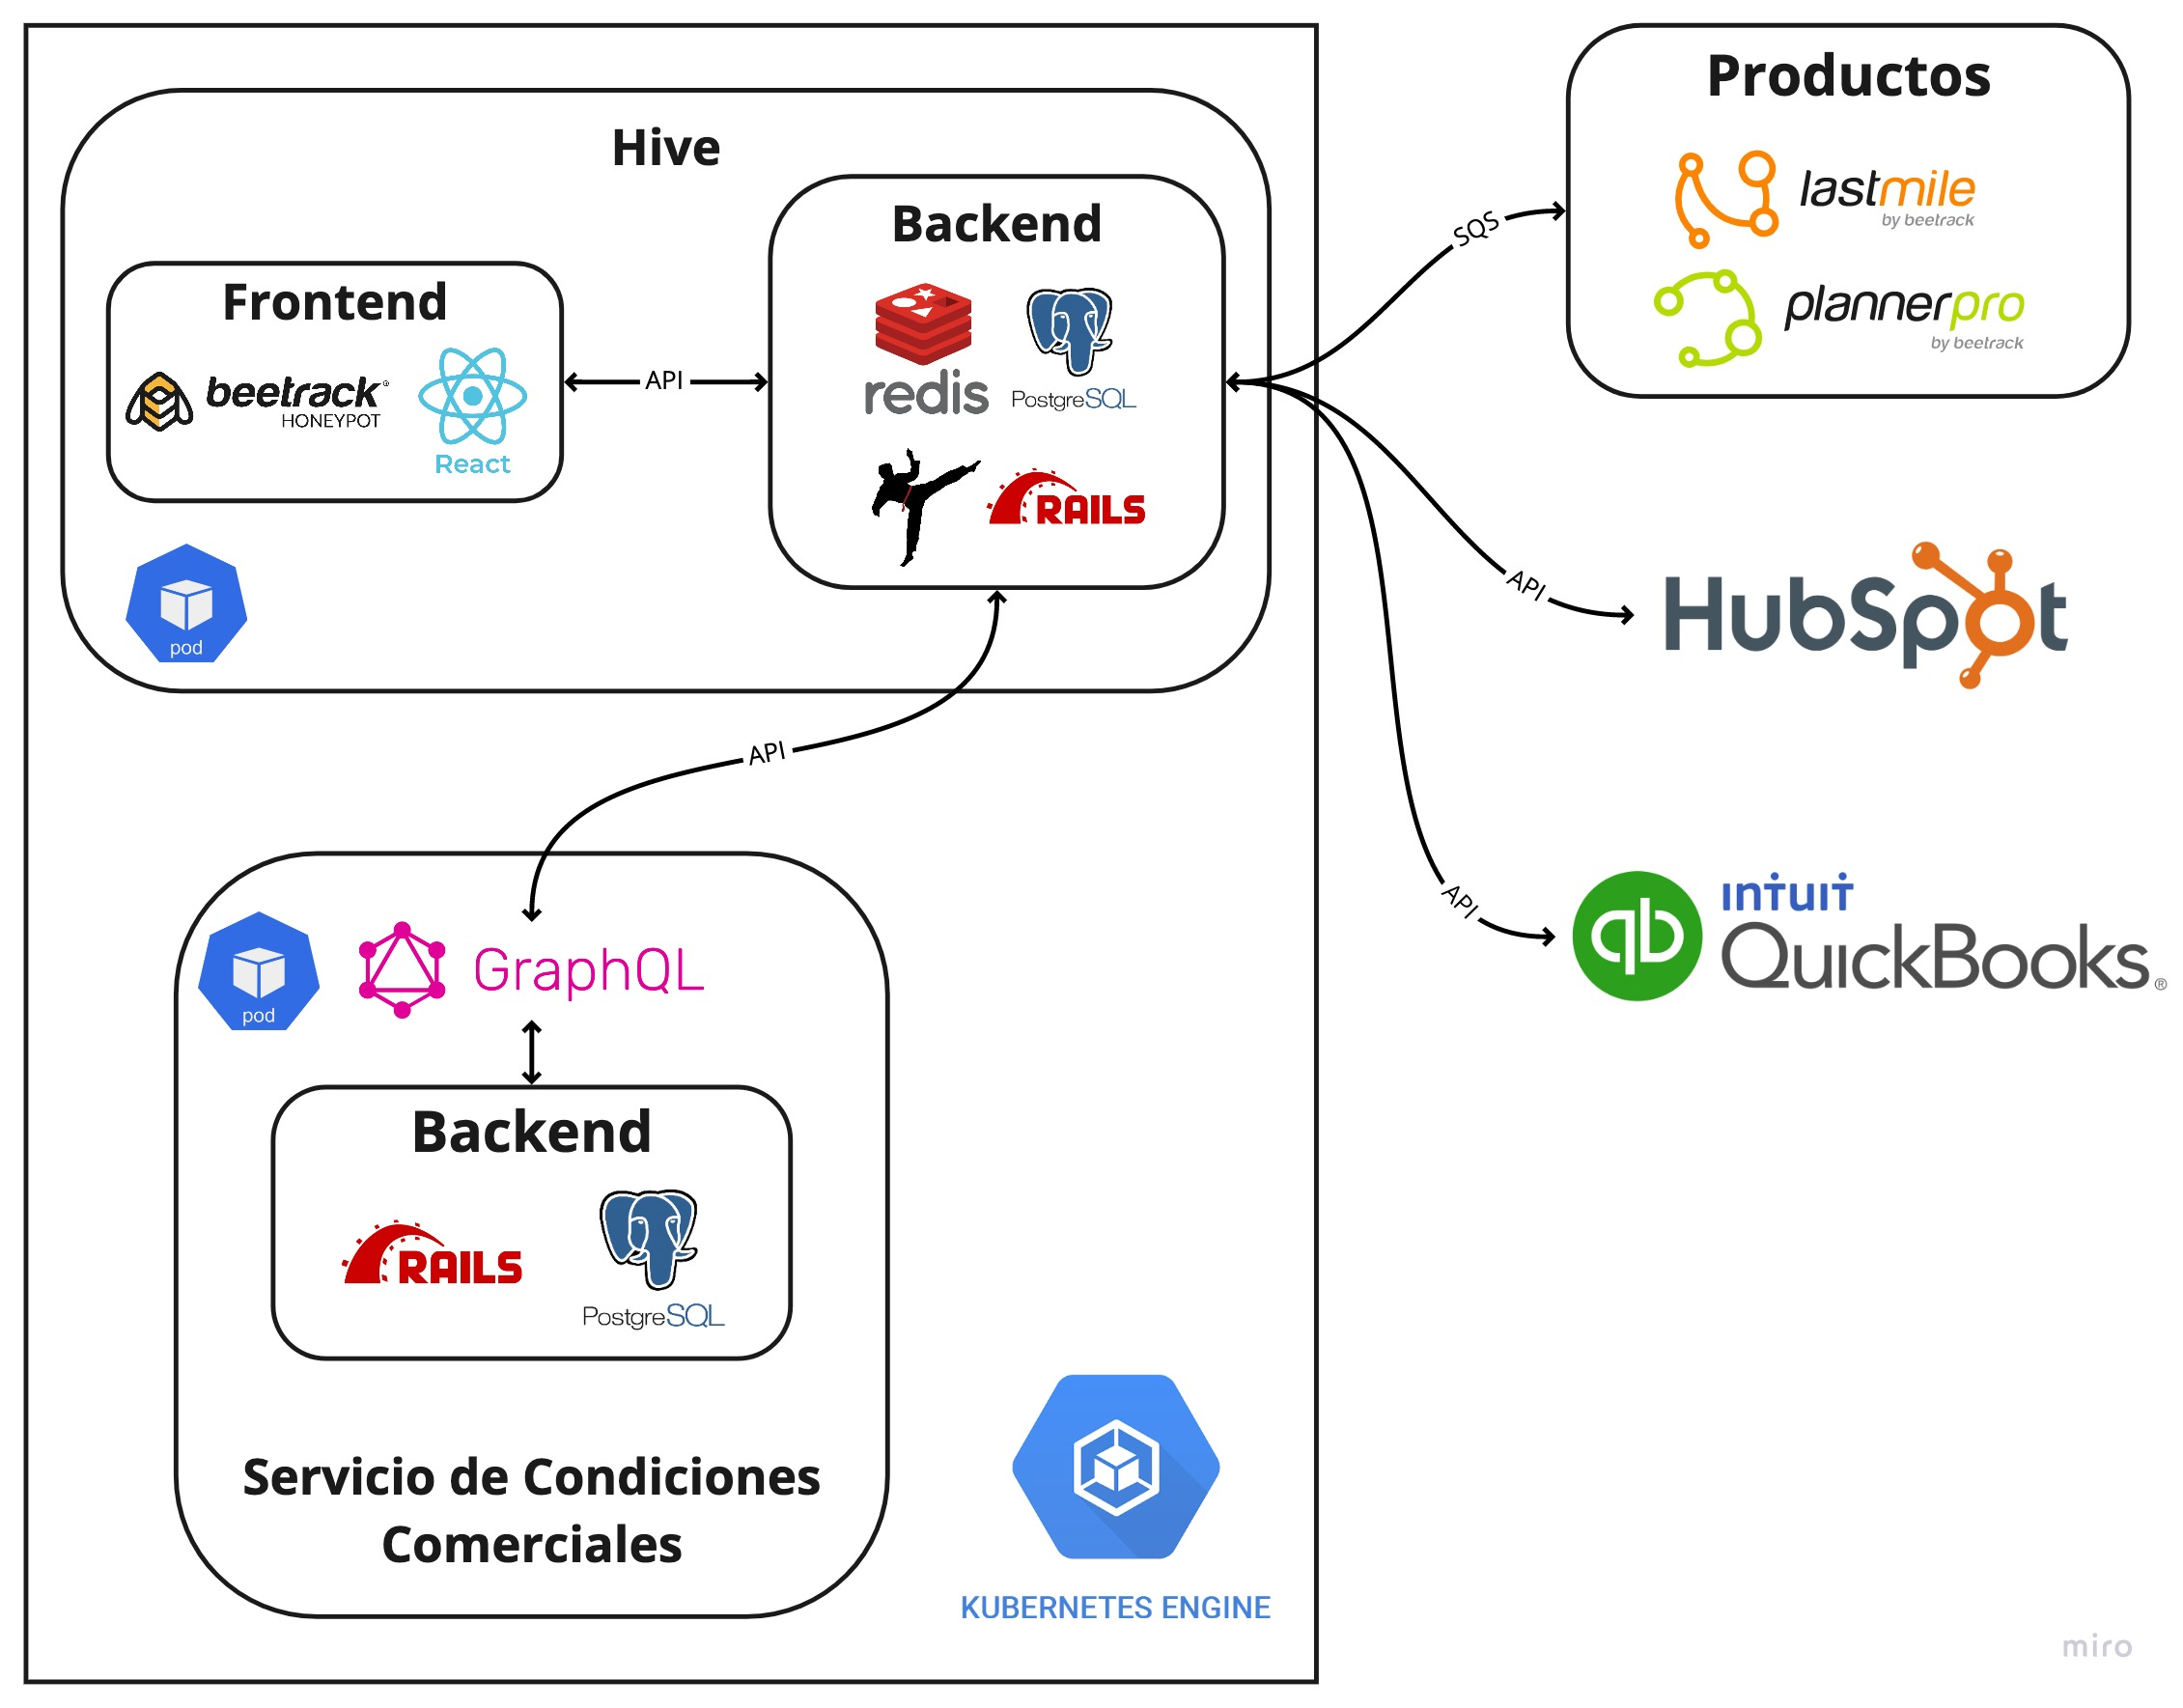
\includegraphics[width=\linewidth]{figures/arquitectura.jpg}
    \caption{Diagrama de tecnologías y arquitectura.}
    \label{fig:arquitectura}
  \end{figure}